\chapter{\acrref{RMS} file format and layout}
    \label{chp:rms}

    \acrref{RMS} files are used to generate random maps that follows some specific pattern. Random maps change each time you play since they are randomly generated starting from a seed $s$. Examples of such maps are \textit{Black Forest} or \textit{Scandinavia}. 
    If you need to create a new type of random map, you need to provide a \code{rms} file. \code{rms} files are written by using a language (called \textit{rms}) created by the developers of \aoe{}\cite{rms:2019}. This section will describes you a \acrref{RMS} file is structured. This section is based on the guide made by Ryan Andrews\cite{rms:2019} and by \cite{zetnus:2019}.

    At high level, a \acrref{RMS} file has 7 basic sections:
    
    \begin{enumerate}
        \item PLAYER\_SETUP;
        \item LAND\_GENERATION;
        \item ELEVATION\_GENERATION;
        \item CLIFF\_GENERATION;
        \item TERRAIN\_GENERATION;
        \item CONNECTION\_GENERATION;
        \item OBJECTS\_GENERATION;
    \end{enumerate}

    As an example, consider \lstref{lst:teamarena} made by vierklee, which represents a random map which create an area where all the teams are located behind procedurally generated walls.

    \lstinputlisting[language={ebnf},label=lst:teamarena,caption={The full source code of the rms file which generates the team maps \dquote{team arena}.}, float, frame=ht]{src/codes/folder-structure.txt}

    At high level, in a \code{rms} file comments follows \code{C} conventions (\ie{} comments start with \dquote{/* } and end with \dquote{ */}). Each section starts with a \textbf{section declaration} and is followed by a section body. Each section declaration follow the regular expression \verb|<[a-zA-Z0-9_]+>\n|. \lstref{lst:rms:regex} specifies the \acrref{EBNF} of the \acrref{RMS} language. The language is case-sensitive and indendation is ignored\cite{zetnus:2019}.

    \lstinputlisting[language={rms},label=lst:rms:regex,caption={EBNF-like statements representing the language of the rms file.}, float, frame=ht]{src/codes/rms-file.txt}

    \section{\acrref{RMS} control flow}

    \subsection{Conditional flow}

    In \acrref{RMS} conditional flow (\ie{} \code{if}, \code{then}, \code{else}) are implemented via the keywords \code{if}, \code{elseif}, \code{else}, \code{endif}. Both \code{elseif} and \code{else} are optiional.
    \lstref{lst:if} shows an example of how to use the conditional flow.

    \begin{lstlisting}[language={rms}, label={lst:if}]
        if FOOBAR
            /* do something when FOOBAR preprocessor directive is specified */
        elseif FOOBAZ
            /* do something when FOOBAZ preprocessor directive is specified */
        else
            /* do something else */
        endif
    \end{lstlisting}

    \subsection{\#include\_drs}

    Include a file located in a given folder. If the filepath is relative, it is relative to the folder \aoeexedir{}\verb|\resources\_common\drs\gamedata_x2| (\eg{} \verb|C:\Program Files (x86)\Steam\steamapps\common\AoE2DE\resources\_common\drs\gamedata_x2|). Inside such a folder, you can several include files that you can use to ease your rms programming. The content of the included file will be dumped as-is in the current file.

    \subsection{\#const}

    \code{C}-like preprocessor. Every time the application see the identifier, it will be replaced by the associated value.

    \begin{lstlisting}[language={rms}, label={lst:const}]
        #const ANSWER 42
    \end{lstlisting}

    For example, in \lstref{lst:const} the statement allows the program to replace \code{ANSWER} with the string 42.

    \section{\acrref{RMS} file sections}

    In the following, we will describe each section. 

    \subsection{PLAYER\_SETUP}

    \paragraph{Player placement}

    In \code{PLAYER\_SETUP} we need to first choose how the players starting position are put in the map. So, you need to put one of the following specifications:

    \begin{itemize}
        \item \textbf{random\_placement}: players are positioned in a circle/oval. This is the default value;
        \item \textbf{grouped\_by\_team}: players are positioned in close proximity to each other. Distance between team members is double the \term{base\_size} used in \term{create\_plater\_lands};
        \item \textbf{direct\_placement}: Allows to manually set the player positions. via create\_land attribute in \term{LAND\_GENERATION}. For example in \lstref{label=rms:manualposition} the first player is positioned in the middle of the map.
        
            \begin{lstlisting}[language=rms,label=rms:manualposition]
                <PLAYER_SETUP>
                direct_placement
                <LAND_GENERATION>
                create_land {
                        terrain_type DESERT
                        land_percent 3
                        land_position 50 50
                        assign_to_player 1
                }
            \end{lstlisting}
        
    \end{itemize}

    If you plan to make the map as a nomad map, you should set the command \term{nomad\_resources}: this will add the cost fo a town center to each player.

    \paragraph{ai\_info\_map\_type}

    Next thing you can set is the \acrref{AI} that \aoe{} will use in the map. You can see as a hint that \aoe{} will use. Such an hint is declared via command \term{ai\_info\_map\_type}. The signature of the command is the one shown in \lstref{rms:setai}, where:

    \begin{lstlisting}[language=rms,label=rms:setai]
        ai_info_map_type MapType IsNomad IsMIchi ShowType
    \end{lstlisting}

    \begin{itemize}
        \item MapType is the map type constants (see \sectionref{subsection:maptype});
        \item IsNomad either 1 or 0: if you plan to make the map as \dquote{nomad}, you are \textbf{required} to set this value to 1;
        \item IsMichi: either 1 or 0: if true a forest will \textbf{completely} separating the players;
        \item ShowType: either 1 or 0: if true, the map type will be shown in the objective tab;
    \end{itemize}

    \subsection{LAND\_GENERATION}

    Place some large areas of terrain in the map. For instance, some maps have some texture representing ground at each player starting location while the rest of the map is filled with grass. This section of the file performs this very feature.

    The first to declare in this section is the type of the terrain you want to have, which can be achieved by using \term{base\_terrain} command. Such a command requires a single input, which should be fetched from the terrain types (see Appendix \ref{subsection:terraintype}).

    Now you need to create large pieces of terrains on the maps. Terrain maps can be used to create a walkable texture at the starting position of a player or a lake in the center like the baltic map\cite{zetnus:2015}.

    \subsubsection{create\_player\_lands}

    The command allows you to create a specific \textbf{land} terrain for \textbf{every} player in the map. This command applies to all the players present in the map. If you want to assign different terrains to different players, consider using \term{create\_land} with \term{assign\_to\_player} instead. The command is optional in the script. If the command can be used multiple times, but every player will have multiple town centers as well as result: this is probably how map \dquote{Budapest} is coded. Note that you give to a player any land, you cannot give to her any starting units or resources as well, so it is \textbf{very important} that each player has at least one starting land.

    \begin{attention}
        \term{create\_player\_lands} cannot be used, due to a bug, alongside \term{direct\_placement}.
    \end{attention}

    \lstref{lst:create-land-player}  shows an example of usage of the command. It will create, for each player, some mass of initial land for the players, where\cite{forgotten-empires:rms-features}:

    \begin{lstlisting}[language=rms,label={lst:create-land-player},caption={Example of usage of \term{create\_player\_lands} in Team Arean by vierklee.}]
        create_player_lands 
        { 
            terrain_type                     GRASS 
            base_size                        19
            land_percent			 5
            clumping_factor                  3
            border_fuzziness                 15
            set_zone_by_team
            other_zone_avoidance_distance    0
            circle_placement
            circle_radius 38
        }
    \end{lstlisting}

    \figref{fig:create-player-lands} shows how teamless map generates each player starting position base.

    \begin{figure}
        \centering
        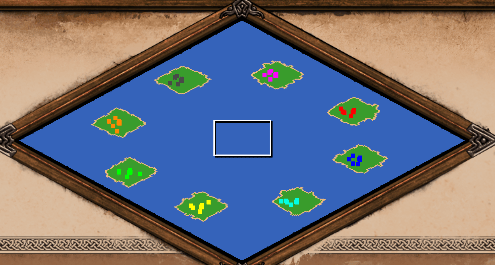
\includegraphics[width=1.0\textwidth]{src/images/create-player-lands}
        \caption{Example of how players are laid out in a map is automatic placement is used.}
        \label{fig:create-player-lands}
    \end{figure}

    The command requires several parameters, which are described next.
    
    \paragraph{\term{terrain\_type}}
    the terrain you want to generate. See \sectionref{subsection:terraintype}.

    \paragraph{\term{land\_percent}}
    Percentage of the total map that the land to create should cover. the number belongs to the range $[0,100]$ (default to 100). If used in \term{create\_player\_lands}, the percentage is divided equally by all the players.

    \paragraph{\term{number\_of\_tiles}}
    Fixed number of tiles that the land should grow by, in addition to the land specified by \term{base\_size}. When \term{behavior\_version} is set to 1, the square origin is included in the total number of tiles, resulting in smaller lands. If used in \term{create\_player\_lands}, the player share the same amount of number of tiles.

    \paragraph{\term{land\_position}}
    Allows you to specify the exact origin point for a land, as a percentage of the total map dimensions. It requires 2 parameters $x$ and $y$ which are, respectively, the x coordinate from the left point to the right and the y coordinate from the bottom to the top of the starting point. You need to satisfy the constraint $x \in [0,100]$, $y \in [0, 99]$. The command cannot be specified when added into \term{create\_player\_lands} or when \term{assign\_to\_player} or \term{assign\_to} is specified into \term{create\_land} (unless \term{direct\_placement} is specified in \term{PLAYER\_SETUP}). The command ignores border restrictions and, if the land is placed outside the border, it will not grow beyond its \term{base\_size}.

    \paragraph{\term{left\_border}, \term{right\_border}, \term{top\_border}, \term{bottom\_border}}
    All needs to satisfy the constraint $x \in [0,97]$, default to $0$. They specify an subset of the map where the land will be put. For instance, this allows the developer to put the players only in the bottom right part of the map (\eg{} in Pilgrims); in \term{create\_player\_lands}, the border coordinates effectively shift the circle where the players are put; when using this function, the created land will have octoagonal shape. For further information, see \url{https://docs.google.com/document/d/e/2PACX-1vR_I1I9u-hI2FFm-EYyjoM_-9dNJFOfTaIgr05wXNbdpv9tI18b6r18ARULy3Jqyvlq6-lc2VjX6xP4/pub#h.xrncn5cs75or}.

    \paragraph{\term{set\_zone\_by\_team}}

    \paragraph{\term{base\_size}}
    It is the radius (in tiles) that each player starting position land will have, in map cells; The bigger it is, the bigger is each player base.

    \paragraph{\term{circle\_radius}}
    It represents the radius of the circle where each player base will be placed. The bigger it is, the more distant each player will be \wrt{}the other ones. The players are put on the circonference of said circle; You need to specify 2 numbers $a$ and $b$: if $a \not = b$, it is produced an ellipse instead of a circle; If $a=b$, $b$ may not be specified.

    \paragraph{\term{circle\_placement}}

    \paragraph{\term{border\_fuzziness}}
    It applies some noise to each player starting land borders ($x \in [0, 100]$). Values near 0 corresponds to perfectly rectangular bases while bigger values tends to create bases with a square-less shape. A good value may be 15; \term{border\_fuzziness} Specifies the extent to which land growth respects the assigned borders. Bigger values means that the borders are fully respected while values near 0 means that the generated area may go beyond the specified border.

    \paragraph{\term{clumping\_factor}}
    Alters the shape of the created land ($x \in [0, 100]$). High values represent rounder lands while low values represents more elongated shapes\cite{zetnus:2019,userpatch15}.

    \paragraph{\term{base\_elevation}}
    elevates the entire land by the specified height ($x \in [0, 9]$). The value is ignore if the terrain is water. Slopes are automatically added to blend the elevation with the sorrounding terrain.

    \paragraph{\term{assign\_to\_player}}
    give ownership of this land to the given player. Allowed values are $x \in [1,8]$ (which are the player lobby positional number). If missing, the land is neutral. Lands assigned to players which are not playing will not be created. Mutually exclusive with \term{assign\_to}.

    \paragraph{\term{assign\_to}}
    Given ownership of this land to the given entity. Mutually exclusive with \term{assign\_to\_player}. It requires 4 additional arguments.

    \begin{enumerate}
        \item AssignTarget, which tells which entity will take ownership of the land. Can be either \term{AT\_PLAYER}, \term{AT\_COLOR} or \term{AT\_TEAM};
        \item Number $x$: represents the specific entity Id of AssignTarget $t \in {0,1,2}$. If $t=\mbox{AT-PLAYER}$ (0), $x \in [1,8]$ (refers to the lobby order); if $t=\mbox{AT-COLOR}$ (1), $x \in [1,8]$ (refers to the player color); If $t=\mbox{AT-TEAM}$ (2), $x \in \{-10,-4,-3-,-2,-1,0,1,2,3,4\}$ (refers to the lobby order of the team, not the number chosen by the team): in this cse is the team 0 refers to unteamed players, while any negative value $x$ represents a player that is not in the team whose lobby order is $-x$. Team -10 is a special team that consists to any player;
        \item Mode $m$: semanticful only if AssignTarget si set to \term{AT\_TEAM}. either -1 or 0. $0$ means the land is assigned randomly in the team while $-1$ means that the land is assigned in an orderly matter;
        \item Flag $f \in [0,3]$. It is a 2-bit biset number. First bit determines if we need to reset players who have already been assigned before startign whiel the second bit tells to avoid remembering the fact that we have assign to a given player this land;
    \end{enumerate}

    When you assign a piece of land to a player, you can also place object owned by such a player. Lands owned by players which are not playing are not generated at all. 

    \paragraph{\term{zone}}

    Allows the land you are creating to be assigned with a particular \textbf{zone id}. Lands which share the same zone id are allwoed to touch eacother when growing. If 2 lands that are going to overlap have different zone ids, will be forbidden to do so: even better, they are garantueed to be distant by \term{other\_zone\_avoidance\_distance}. The command is mutually exclusive with \term{set\_zone\_by\_team} and with \term{set\_zone\_randomly}. Lands created with \term{create\_player\_lands} have their own unique zone id, while all lands created with \term{create\_land} share the same zone id.

    \begin{attention}
        Zone 99 will crash the game.
    \end{attention}

    \paragraph{\term{set\_zone\_by\_team}}

    Assign the same zone to all the members of the same team. Usage is recommended only in \term{create\_player\_lands}.

    \paragraph{\term{set\_zone\_randomly}}

    TODO

    \paragraph{\term{other\_zone\_avoidance\_distance}}
    Number of cells that each starting player position needs be distant from the other zones. If such a value is set to 0, each starting position base may overlap with others (like in Team Arena by vierklee).

    \paragraph{\term{min\_placement\_distance}}

    \paragraph{\term{land\_id}}

    Assign a numeric label to a land, which can later be used to place object specifically on that land via \term{place\_on\_specific\_land\_id} command. Multiple lands may share the same ID. The commands needs to be used after \term{assign\_to\_player} or \term{assign\_to}, since they will reset the ID.

    \paragraph{create\_land}

    Creates a single piece of land which is owned by no players. Hence it can be used to place neutral mass of lands (\eg{} shared continent or shared{} center lakes, like in Baltic).
    As an example, consider \lstref{lst:create-land}: the example create a lake centered in the middle of the map. The lake itself covers 20\% of the map

    \begin{lstlisting}[language=rms,label={lst:create-land},caption={Example of usage of \term{create\_land} in Team Arean by vierklee.}]
        create_land
        { 
            terrain_type WATER
            land_percent 20
            land_position 50 50
        }
    \end{lstlisting}

    \subsection{\term{CLIFF\_GENERATION}}

    Thanks to this section, cliffs are added in the map\cite{aok:cliffs, zetnus:2015}.
    Cliffs are generated \textit{after} lands but \textit{before} terrain. If the section declaration is left empty, some cliff are still generated on the map.
    To further customize the cliffs, you need to input other commands.

    \paragraph{\term{min\_number\_of\_cliffs}}

    The mininum number of cliffs to generate. It requires the number of minimum cliffs to generate. For instance, in \lstref{lst:minimumnumberofcliffs} we generate at least 10 cliffs.

    \begin{lstlisting}{language=rms, label={lst:minimumnumberofcliffs}}
        <CLIFF_GENERATION>
        min_number_of_cliffs 10
    \end{lstlisting}

    \begin{warning}
        If you put a large number of cliffs, the number of cliffs will be truncated if there is not enough space in the map.
    \end{warning}

    \paragraph{\term{max\_number\_of\_cliffs}}

    The maximum number of cliffs to generate. It requires the number of maximum cliffs to generate. For instance, in \lstref{lst:minimumnumberofcliffs} we generate at most 10 cliffs.

    \begin{lstlisting}{language=rms, label={lst:minimumnumberofcliffs}}
        <CLIFF_GENERATION>
        max_number_of_cliffs 10
    \end{lstlisting}

    \paragraph{\term{min\_distance\_cliffs}}

    The minimum number of \textbf{cliff unit} that separates one cliff to another one. It accepts a single number $x \geq 0$, whose default value is 2.

    \begin{definition}
        A cliff unit corresponds to 3 map tiles.
    \end{definition}

    \paragraph{\term{min\_length\_of\_cliff} and \term{max\_length\_of\_cliff}}

    The minimum (and the maximum) length of a generic cliff. Note that you are required to satisfy $min \geq max, min \geq 0, max \geq 0$.

    \paragraph{\term{cliff\_curliness}}

    Determines how much the cliffs tends to change directions ($x \in [0, 100]$). At 0, cliffs will be very straight and at 100 they will be extremely twisted. For example in \lstref{lst:cliffcurliness} we will generate exactly 20 cliffs, which are a bit \dquote{curly}.

    \begin{lstlisting}{language=rms, label={lst:cliffcurliness}}
        <CLIFF_GENERATION>
        min_number_of_cliffs 20
        max_number_of_cliffs 20
        cliff_curliness  10
    \end{lstlisting}

    \subsection{\term{TERRAIN\_GENERATION}}

    Replace terrains with other terrains. It is usually used to place clumps of forest, adding textures to make the map more nice, adding small lakes into chunks of forests and so on. The main command you should use here is \term{create\_terrain}, although you can also use the following commands:

    \begin{itemize}
        \item \term{color\_correction};
    \end{itemize}



    \subsubsection{\term{color\_correction}}

    Specify a color correction to the whole map. Within the game, such an option is available via \dquote{Map Lightning}. The command accepts a single argument $x$, which can be one of the following: \code{CC\_AUTUMN}, \code{CC\_WINTER}, \code{CC\_JUNGLE}, \code{CC\_DESERT}.

    \subsubsection{\term{create\_terrain} TERRAIN}

    Create a single piece of terrain. Depending on which terrain you add in the map, the behavior may change. It accepts a lot of arguments, hence we will deal with them in several paragraphs.

    \paragraph{\term{base\_terrain} TERRAIN}

    It performs like the argument in the land generation.

    \begin{attention}
        Due to a bug, the value does not default to \term{GRASS}.
    \end{attention}

    \paragraph{\term{terrain\_mask} NUM}

    Enables terramin masking or layering for the terrain being created. The terrain to add inherits all properties, placement restrictions, automatic objects (\eg{} trees for forest terrains or minimap color) from the base terrain. This function is great to blend terrains in order to create more realistic and aesthetically pleasant maps. The only argument is the layer number, which can either 0 (no masking), 1 or 2. Setting the layer to 1 means that the new terrain is masked \textit{above} the base terrain ajnd inherits its properties. On the other hand, setting the layer to 2 means that the terrain to ad is placed \textit{below} the base terrain: in this case the base terrain will inherits the properties from the terrain just added.

    \begin{note}
        Terrain will have animated water if any of the terrains are water.
    \end{note}

    \paragraph{\term{spacing\_to\_other\_terrain\_types} NUM}

    Minimum distance that this terrain will stay away from other terrain types. It requires a number $x \geq 0$ (default to 0). This value considers only the terrains already present. The command will ignore terrain sharing the same terrain type. If \term{set\_flat\_terrain\_only}, the terrain will distance that the terrain will stay away from slopes.

    \paragraph{\term{set\_flat\_terrain\_only}}

    Command the map generation to avoid slopes tiles by the distance specified by the only argument $x$, $x \geq 1$. \lstref{lst:flatterrainonly} shows an example where the generator creates a hill where the bottom and the top are desert, but the slopes are grass.

    \begin{lstlisting}[language={rms},label={lst:flatterrainonly}]
        <ELEVATION_GENERATION>
        create_elevation 7 {
            base_terrain GRASS
            number_of_tiles 3000
            number_of_clumps 1
        }

        <TERRAIN_GENERATION>
        create_terrain DESERT {
            base_terrain GRASS
            land_percent 100
            number_of_clumps 9320
            spacing_to_other_terrain_types 1
            set_flat_terrain_only
        }
    \end{lstlisting}

    \paragraph{\term{land\_percent} NUM}

    Percentage of the total map allocated to this \term{create\_terrain} command. If \term{number\_of\_clumps} is specified, this value is divided equally among the clumps. \lstref{lst:createterrain} contains an example where a a desert covers 50\% of the map. The terrain will only be replaced where the appropriate \term{base\_terrain} or \term{base\_layer} is present, and will only replace the specified number of individual clumps, so it will not necessarily fill 100\% of the map if set to 100.

    \begin{lstlisting}[language={rms},label={lst:createterrain}]
        <TERRAIN_GENERATION>
        create_terrain DESERT {
            base_terrain GRASS
            land_percent 50
        }
    \end{lstlisting}

    \paragraph{\term{number\_of\_tiles} NUM}

    Total time count allocate dto this \term{create\_terrain} command. If \term{number\_of\_clumps} is specified, this value is divided equally among the clumps.

    \paragraph{\term{number\_of\_clumps} NUM}

    TODO

    \paragraph{\term{clumping\_factor} NUM}

    TODO

    \paragraph{\term{set\_scale\_by\_size}}

    Scales \term{number\_of\_tiles} to the map size. Unscaled value refers to a 100x100 map (see: \tblref{tbl:size}). If you see a script scaling by both size and groups, only the final attribute will apply! If you want to scale by both groups and size, use \term{set\_scale\_by\_groups} instead. \lstref{lst:setscalebysize} contains an example where the map generator creates 4 lakes which become larger on larger maps; on a small map this will be 4 clumps with a total of $400 \cdot 2.1 = 840$ tiles. The command is mutually exclusive with \term{set\_scale\_by\_groups}.

    \begin{lstlisting}[language={rms},label={lst:setscalebysize}]
        <TERRAIN_GENERATION>
        create_terrain WATER {
            base_terrain GRASS
            number_of_clumps 4
            number_of_tiles 400
            set_scale_by_size
        }
    \end{lstlisting}

    \paragraph{\term{set\_scale\_by\_groups}}

    Scales \term{number\_of\_clumps} to the map size. Unscaled value refers to a 100x100 map (see \tblref{tbl:size}). If you see a script scaling by both size and groups, only the final attribute will apply! When used with \term{number\_of\_tiles}, the total tiles are also scaled to map size as well (but only for terrains, not for elevation). For example, \lstref{lst:setscalebygroups} allows to  Create 400 tiles worth of lakes, with the number of lakes \textit{and} the total number of tiles scaling to map size. On a small map this will be 4x2.1 = 8 clumps with a total of $400 \cdot 2.1 = 840$ tiles.

    \begin{lstlisting}[language={rms},label={lst:setscalebygroups}]
        <TERRAIN_GENERATION>
        create_terrain WATER {
            base_terrain GRASS
            number_of_clumps 4
            number_of_tiles 400
            set_scale_by_groups
        }
    \end{lstlisting}

    \paragraph{\term{set\_avoid\_player\_start\_areas}}

    \paragraph{\term{height\_limits} NUM NUM}

    The terrain will only be placed on tiles of height between min and max (inclusive). For most purposes, values between 0 and 7 are useful, where 0 being the standard non-elevated height and 7 being the max height that can be produced by \term{create\_elevation}. For example \lstref{lst:heightslimits} allows you to create a hill and place desert terrain only on the slopes.

    \begin{lstlisting}[language={rms},label={lst:heightslimits}]
        <ELEVATION_GENERATION>
            create_elevation 7 {
            base_terrain GRASS
            number_of_tiles 3000
            number_of_clumps 1
        }

        <TERRAIN_GENERATION>
            create_terrain DESERT {
            base_terrain GRASS
            land_percent 100
            number_of_clumps 9320
            height_limits 1 6
        }
    \end{lstlisting}

    \subsection{\term{CONNECTION\_GENERATION}}

    The section allows to replace terrains with other terrains, specifically along a given pah between the origins of lands. Used to create roads between players, shallows area across rivers and to ensure that forests do not completely separate players. If a connection provided by the \acrref{RMS} file is not possible, it is skipped.  Each commands creates several connections between points and perform an action over the terrains.

    Each command can be associated to several attributes, which are described below:

    \paragraph{\term{default\_terrain\_replacement} TERRAIN}

    Replace all the terrains in the connections with the specified terrain.

    \paragraph{\term{replace\_terrain} TERRAIN1 TERRAIN2}

    If the terrain \code{TERRAIN1} is part of a connection, replace it with the terrain \code{TERRAIN2}. Can be used multiple times for different terrains.

    \begin{attention}
        The terrain \code{TERRAIN1} refers to the terrain that the map generator detects it at the beginning of the \code{CONNECTIOn\_GENERATION} section.
    \end{attention}

    \paragraph{\term{terrain\_cost} TERRAIN NUM}

    The cost of having the connection run through the specified terrain. This allows the path finding algorithm \cite{dijkstra1959a} to alter the optimal solution. If the terrain is the one \code{TERRAIN}, the cost of such edges are temporary set to \code{NUM} instead of 1. $NUM > 0$. \lstref{lst:replacecost} shows an example of how to use this attribute.

    \begin{lstlisting}[language={rms},label={lst:replacecost}]
        <CONNECTION_GENERATION>
        create_connect_all_players_land {
            replace_terrain GRASS ROAD
            replace_terrain FOREST LEAVES
            replace_terrain WATER SHALLOW
            replace_terrain MED_WATER SHALLOW
            replace_terrain DEEP_WATER SHALLOW
            terrain_cost GRASS 1
            terrain_cost FOREST 7
            terrain_cost WATER 7
            terrain_cost MED_WATER 12
            terrain_cost DEEP_WATER 15
        }
    \end{lstlisting}

    \paragraph{\term{terrain\_size} TERRAIN NUM NUM}

    When a connection passes through a tile of the specified terrain, the area within radius +/- variance will be subject to \term{replace\_terrain} or \term{default\_terrain\_replacement} and terrains will be replaced accordingly. \lstref{lst:terrainsize} shows an example of how to use this attribute: the roads are slightly larger. The first argument represents the radius of the road we are building while the second parameter represents the variance of the radius of the road we are building.

    \begin{lstlisting}[language={rms},label={lst:terrainsize}]
        <CONNECTION_GENERATION>
        create_connect_all_players_land {
            replace_terrain GRASS ROAD
            replace_terrain WATER SHALLOW
            terrain_size GRASS 1 1
            terrain_size WATER 3 1
        }
    \end{lstlisting}

    \subsubsection{\term{create\_connect\_all\_players\_land}}

    Create several connection in order to make sure that all lands of players (both the starting ones and the ones assigned to them) are reachable. Each connection edge $(u,v)$, where $u,v$ represent two players. An example of the connection generated are shown in \figref{fig:createconnectallplayersland}.

    \begin{figure}[ht]
        \centering
        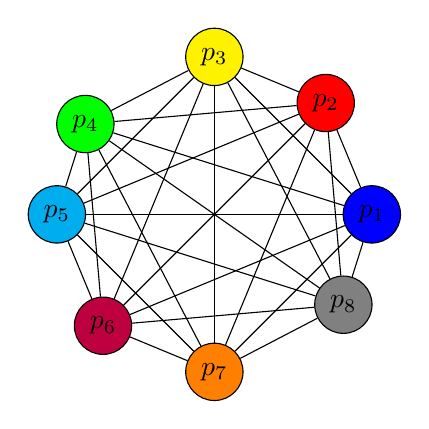
\begin{tikzpicture}

            \node[shape=circle, fill=blue, draw=black] (P1) at (0:2cm) {$p_1$};
            \node[shape=circle, fill=red, draw=black] (P2) at (45:2cm) {$p_2$};
            \node[shape=circle, fill=yellow, draw=black] (P3) at (90:2cm) {$p_3$};
            \node[shape=circle, fill=green, draw=black] (P4) at (145:2cm) {$p_4$};
            \node[shape=circle, fill=cyan, draw=black] (P5) at (180:2cm) {$p_5$};
            \node[shape=circle, fill=purple, draw=black] (P6) at (225:2cm) {$p_6$};
            \node[shape=circle, fill=orange, draw=black] (P7) at (270:2cm) {$p_7$};
            \node[shape=circle, fill=gray, draw=black] (P8) at (325:2cm) {$p_8$};
            
            \path[-.](P1) edge node[left] {} (P2);
            \path[-.](P1) edge node[left] {} (P3);
            \path[-.](P1) edge node[left] {} (P4);
            \path[-.](P1) edge node[left] {} (P5);
            \path[-.](P1) edge node[left] {} (P6);
            \path[-.](P1) edge node[left] {} (P7);
            \path[-.](P1) edge node[left] {} (P8);

            \path[-.](P2) edge node[left] {} (P3);
            \path[-.](P2) edge node[left] {} (P4);
            \path[-.](P2) edge node[left] {} (P5);
            \path[-.](P2) edge node[left] {} (P6);
            \path[-.](P2) edge node[left] {} (P7);
            \path[-.](P2) edge node[left] {} (P8);

            \path[-.](P3) edge node[left] {} (P4);
            \path[-.](P3) edge node[left] {} (P5);
            \path[-.](P3) edge node[left] {} (P6);
            \path[-.](P3) edge node[left] {} (P7);
            \path[-.](P3) edge node[left] {} (P8);

            \path[-.](P4) edge node[left] {} (P5);
            \path[-.](P4) edge node[left] {} (P6);
            \path[-.](P4) edge node[left] {} (P7);
            \path[-.](P4) edge node[left] {} (P8);

            \path[-.](P5) edge node[left] {} (P6);
            \path[-.](P5) edge node[left] {} (P7);
            \path[-.](P5) edge node[left] {} (P8);

            \path[-.](P6) edge node[left] {} (P7);
            \path[-.](P6) edge node[left] {} (P8);

            \path[-.](P7) edge node[left] {} (P8);
        \end{tikzpicture}
        \caption{Connections generated by \term{create\_connect\_all\_players\_land} command.}
        \label{fig:createconnectallplayersland}
    \end{figure}

    As an example of how to use this command, you see \lstref{lst:connectionplayers}.

    \begin{lstlisting}[language={rms}, label={lst:connectionplayers}, caption={Example showing how you can connect all players with dirt.}]
        <LAND_GENERATION>
        create_player_lands {
            terrain_type DESERT
            number_of_tiles 100
        }

        <CONNECTION_GENERATION>
            create_connect_all_players_land {
            default_terrain_replacement DIRT
        }
    \end{lstlisting}

    \subsubsection{\term{create\_connect\_teams\_lands}}

    Create several connections. Each connection edge $(u,v)$, where $u,v$ represent two players starting position belonging to the same team. An example of the connection generated are shown in \figref{fig:createconnectteamslands}. The road generated may go into enemy teams or neutral teams as well, if the connection is the optimal one.

    \begin{figure}[ht]
        \centering
        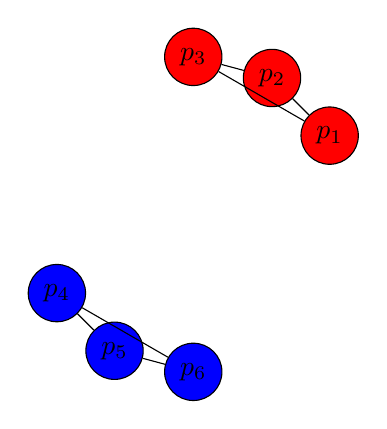
\begin{tikzpicture}

            \node[shape=circle, fill=red, draw=black] (P1) at (30:2cm) {$p_1$};
            \node[shape=circle, fill=red, draw=black] (P2) at (60:2cm) {$p_2$};
            \node[shape=circle, fill=red, draw=black] (P3) at (90:2cm) {$p_3$};
            \node[shape=circle, fill=blue, draw=black] (P4) at (210:2cm) {$p_4$};
            \node[shape=circle, fill=blue, draw=black] (P5) at (240:2cm) {$p_5$};
            \node[shape=circle, fill=blue, draw=black] (P6) at (270:2cm) {$p_6$};
            
            \path[-.](P1) edge node[left] {} (P2);
            \path[-.](P2) edge node[left] {} (P3);
            \path[-.](P3) edge node[left] {} (P1);

            \path[-.](P4) edge node[left] {} (P5);
            \path[-.](P5) edge node[left] {} (P6);
            \path[-.](P6) edge node[left] {} (P4);
        \end{tikzpicture}
        \caption{Connections generated by \term{create\_connect\_teams\_lands} command. Only connections between teammates are generated.}
        \label{fig:createconnectteamslands}
    \end{figure}

    \lstref{lst:connectionteam} shows an example where the command is used to replace the terrain to \term{ROAD}.

    \begin{lstlisting}[language={rms}, label={lst:connectionteam}, caption={Example showing how you can connect teammates with roads.}]
        <LAND_GENERATION>
        create_player_lands {
            terrain_type DESERT
            number_of_tiles 100
        }

        <CONNECTION_GENERATION>
        create_connect_all_players_land {
            replace_terrain FOREST ROAD
            replace_terrain GRASS ROAD
        }
    \end{lstlisting}

    \subsubsection{\term{create\_connect\_all\_lands}}

    Connections will be generated in order to connect all the lands present on the map.

    \subsubsection{\term{create\_connect\_same\_land\_zones}}

    Apparently the same of \term{create\_connect\_all\_lands}.

    \subsubsection{\term{create\_connect\_to\_nonplayer\_land}}

    Connect all player lands to all neutral lands, but do not directly generate connections between individual players.

    \begin{attention}
        After calling this command, all other connection commands appearing afterwards will not work anymore.
    \end{attention}

    \subsection{\term{OBJECTS\_GENERATION}}

    This section deals when placing buildings, units, resources, animals, straggler trees, decorations and other stuffs. Objects are placed in the same order as they appear in the \acrref{RMS} file. Normally, each tile can contains at most 1 object. If the object cannot be placed, it is not generated at all. The command that places objects is performed via \term{create\_object} command.

    \begin{note}
        Consider placing first the most important objects.
    \end{note}

    The attributes of \term{create\_object} are shown below (since they are many).

    \paragraph{\term{number\_of\_objects} NUM}

    Number of objects to places in the whole map. The num needs to $x \in [1, 9320]$. \lstref{lst:numerofobjects} allows to generate 10 batches of gold mines in the whole map.

    \begin{lstlisting}[language={rms}, label={lst:numerofobjects}, caption={Example showing how you can create object in the whole map.}]
        <OBJECTS_GENERATION>
        create_object GOLD {
            number_of_objects 10
        }
    \end{lstlisting}

    \paragraph{\term{number\_of\_groups} NUM}

    Place a number of objects grouped together. Note that the total number of objects added is $n \cdot g$, where $n$ is \term{number\_of\_objects} and $g$ is the \term{number\_of\_groups}. \lstref{lst:numerofgroups} allows to generate 20 groups of gold mines, each with 5 patches of gold.

    \begin{lstlisting}[language={rms}, label={lst:numerofgroups}, caption={Example showing how you can create object in the whole map, grouped together.}]
        <OBJECTS_GENERATION>
        create_object GOLD {
            number_of_objects 5
            number_of_groups 20
        }
    \end{lstlisting}

    \paragraph{\term{groups\_variance} NUM}

    The \term{number\_of\_objects} is randomly varied up to $\pm$ the amount specified. Note that this is not the mathematically variance, but the standard deviation.
    Each group generated has a different number of objects. \lstref{lst:groupvariance} allows to generate 10 groups of gold mines, each with patches of $5 \pm 3$ gold.

    \begin{lstlisting}[language={rms}, label={lst:groupvariance}, caption={Example showing how you can create different groups of object in the whole map, with different number of objects in each group.}]
        <OBJECTS_GENERATION>
        create_object GOLD {
            number_of_objects 5
            number_of_groups 10
            group_variance 3
            set_tight_grouping
        }
    \end{lstlisting}

    \paragraph{\term{resource\_delta} NUM}

    TODO

    \paragraph{\term{second\_object} OBJECT}

    TODO

    \paragraph{\term{set\_scaling\_to\_map\_size}}

    TODO 

    \paragraph{\term{set\_scaling\_to\_player\_number}}

    TODO

    \paragraph{\term{set\_place\_for\_every\_player}}

    Place the object(s) as a personal object for each player (actually for each player land). Objects that cannot be owned by players (\eg{} boar, gold, trees, and so on) also require \term{set\_gaia\_object\_only} to be placed for every player.

    Only works for player lands or lands assigned to players. Disabled by \term{land\_id}. Objects will only be placed where they are not separated from the origin of their land by a terrain they are restricted on.

    This means that on islands your resources will only end up on your own island. It also means that player gold mines on acropolis can only be placed on the hilltops, because gold is restricted from the rock terrain. Water objects (docks/boats) CAN be placed if the player land is made of a dirt terrain type. Terrain restrictions can be bypassed by using a placeholder and \term{second\_object}. Even though road terrains are restricted for resources, they do not form a separation the way other terrains do. \lstref{lst:setplaceforeveryplayer} allows to give every player their starting villagers.

    \begin{lstlisting}[language={rms}, label={lst:setplaceforeveryplayer}, caption={Example showing how you can give to each player a single villager.}]
        create_object VILLAGER {
            set_place_for_every_player
            min_distance_to_players 6
            max_distance_to_players 7
        }
    \end{lstlisting}

    \paragraph{\term{place\_on\_specific\_land\_id} NUM}

    TODO

    \paragraph{\term{set\_gaia\_object\_only}}

    Use it alongside \term{set\_place\_for\_every\_player} to place gaia objects on a per-player basis. Muyst be used when placing neutral units (\eg{} stone, deer, boars). Units and buildings will permanently join the player who first finds them unless \term{set\_gaia\_unconvertible} is specified. Gaia building architecture (in case of buildings) can be specified via \term{set\_gaia\_civilization}.

    \begin{lstlisting}[language={rms}, caption={Give every player 4 gaia sheep close to their starting town.}]
        <OBJECTS_GENERATION>
        create_object SHEEP {
            number_of_objects 4
            set_loose_grouping
            set_gaia_object_only
            set_place_for_every_player
            min_distance_to_players 7
            max_distance_to_players 8
        }
    \end{lstlisting}

    \paragraph{\term{set\_gaia\_unconvertible}}

    TODO

    \paragraph{\term{group\_placement\_radius} NUM}

    Specify the number of tiles out from the central tile that objects belonging to the same group may spawn ($x > 0$, default to 3). Active only  when grouping behavior is specified. 

    \paragraph{\term{set\_tight\_grouping}}

    TODO

    \paragraph{\term{set\_loose\_grouping}}

    TODO

    \paragraph{\term{terrain\_to\_place\_on} TERRAIN}

    The object(s) will only be placed on the specified terrain. The argument passes can be set 

    \begin{lstlisting}[language={rms}, caption={Example where place decorative rocks on a central desert..}]
        <LAND_GENERATION>
        create_land {
            terrain_type DESERT
            number_of_tiles 500
            land_position 50 50
        }

        <OBJECTS_GENERATION>
            create_object ROCK {
            number_of_objects 300
            terrain_to_place_on DESERT
        }
    \end{lstlisting}

    \paragraph{\term{layer\_to\_place\_on} TERRAIN}

    TODO

    \paragraph{\term{place\_on\_forest\_zone}}

    TODO

    \paragraph{\term{avoid\_forest\_zone} NUM}

    TODO

    \paragraph{\term{avoid\_cliff\_zone} NUM}

    TODO

    \paragraph{\term{min\_distance\_to\_players} NUM and \term{max\_distance\_to\_players} NUM}

    Minimum distance (in tiles) from the origin of player lands where that the object can be placed. It is not necessary to specify both attributes. If the objects are grouped, distance refers to the center of the group, not the individual members. When used with \term{place\_on\_specific\_land\_id}, distances refer to that specific land. When used without \term{set\_place\_for\_every\_player} or \term{place\_on\_specific\_land\_id}, maximum distance has no effect.
    
    \begin{attention}
        There is a bug in \aoe{} such that if distances are very constrained (\ie{} $min=max$), objects are noticeably biased towards being placed in the west (\ie{} starting villagers). Furthermore, when used with \term{set\_place\_for\_every\_player} or \term{place\_on\_specific\_land\_id}, minimum distance applies to \textbf{all} lands, not just player lands (or the specific ID).
    \end{attention}

    \begin{lstlisting}[language={rms}, caption={Place the starting scout at a distance of 7-9 tiles}]
        <OBJECTS_GENERATION>
        create_object SCOUT {
            set_place_for_every_player
            min_distance_to_players 7
            max_distance_to_players 9
        }
    \end{lstlisting}


    \paragraph{\term{max\_distance\_to\_other\_zones} NUM}

    TODO

    \paragraph{\term{min\_distance\_group\_placement} NUM}

    Minimum distance in tiles that individual objects of the same \term{create\_object} command, and \textit{all} future objects, must stay away from each object.

    Best used with small values, to keep different resources from being directly next to each other. To scatter objects from the same command far away from each other, use \term{temp\_min\_distance\_group\_placement}. If the objects are grouped, distance applies to whole groups, and refers to the center.

    \begin{lstlisting}[language={rms}, caption={Give each player two sets of forages and make them avoid each other by 4 tiles, and keep all future objects 4 tiles away.}]
        <OBJECTS_GENERATION>
        create_object FORAGE {
            number_of_objects 7
            number_of_groups 2
            set_tight_grouping
            set_place_for_every_player
            set_gaia_object_only
            min_distance_to_players 8
            max_distance_to_players 10
            min_distance_group_placement 4
        }
    \end{lstlisting}

    \paragraph{\term{temp\_min\_distance\_group\_placement} NUM}

    TODO

    \paragraph{\term{find\_closest}}

    TODO

    \paragraph{\term{force\_placement}}

    TODO

    \paragraph{\term{actor\_area} ID}

    TODO

    \paragraph{\term{actor\_area\_radius} NUM}

    TODO

    \paragraph{\term{actor\_area\_to\_place\_in} ID}

    TODO

    \paragraph{\term{avoid\_actor\_area} ID}

    TODO

    \paragraph{\term{avoid\_all\_actor\_areas}}

    TODO

    \paragraph{\term{max\_distance\_to\_players} NUM}

    \section{Functions}

    The section provides the utility functions you can use within \acrref{RMS} file.

    \subsection{Random}

    If you need to generate a random number, use \code{rnd} function.
    \begin{enumerate}
        \item min: the minimum number that the function can generate;
        \item max: the maximum number that the function can generate;
    \end{enumerate}
    It generates a number $x \in [min,max]$. The example in \lstref{rms:rnd} yields numbers in the set $\{5,6,7\}$.

    \begin{lstlisting}[language=rms,label=rms:rnd]
        foobar rnd(5,7)
    \end{lstlisting}

    \subsection{Choose a randomly chosen scenario}

    If you need to perform a different command depending on a randomly generated number, you can use the construct \term{start\_random}, \term{end\_random}, as shown in \lstref{rms:startrandom}: such a construct will set \code{FOO} to 3 in the 25\% of the cases, 4 in the 25\% of the cases and 5 in the remainder 50\% of cases.

    \begin{lstlisting}[language=rms,label=rms:startrandom]
        start_random
            percent_chance 25 #const FOO 3
            percent_chance 25 #const FOO 4
            percent_change 50 #const FOO 5
        end_random
    \end{lstlisting}

    \section{Inherited constants from the environment}

    When building a map, it is possible to use conditional in order to check what are the parameters of the map that we need to generate. For example, you may want to obtain how big the map to generate is (\eg{} tiny, normal, ludicruous). To do so, you can check whether one of the macro in \tblref{tbl:mapsizemacro} is defined.

    \begin{table}
        \centering
        \begin{tabular}{ll}
            \toprule
            Map size name & Macro to check \\
            \midrule
            Tiny & TINY\_MAP \\
            Tiny & SMALL\_MAP \\
            Tiny & MEDIUM\_MAP \\
            Tiny & LARGE\_MAP \\
            Tiny & HUGE\_MAP \\
            Tiny & GIGANTIC\_MAP \\
            Tiny & LUDIKRIS\_MAP \\
            \bottomrule
        \end{tabular}
        \caption{Macro to check if you want to detect the map size}
        \label{tbl:mapsizemacro}
    \end{table}

    \section{Popular included files}

    \subsection{thebr\_setup.inc}

    Seems empty

    \subsection{F\_seasons.inc}

    You can include \code{F\_seasons.inc} file. Such a file changes the texture of the random map, depending on which macros are defined: \tblref{tbl:seasons} shows which macros should be define in order to tweak the aesthetic of the map. Usually you need to first define one of the macros and then import \code{F\_seasons.inc} (via \term{include\_drs}).

    \begin{landscape}
        \centering % Center table
        \begin{tabular}{ll}
            \toprule
            Macro   & Description \\
            \midrule
            \term{PH\_ALPINE} & \\
            \term{PH\_ALPINE\_B} & No leaves allowed \\
            \term{PH\_SPRING} & \\
            \term{PH\_SPRING\_C} & \\
            \term{PH\_MEDISOUTH} & \\
            \term{PH\_SPRING\_B} &  No Leaves allowed \\
            \term{PH\_TROPHICALSOUTH} & \\
            \term{PH\_TROPHICALSOUTH\_B} & Jungle read instead of grass 2 \\
            \term{PH\_TROPHICALEAST} & \\
            \term{PH\_DESERT} & \\
            \term{PH\_AFRICAN} & \\
            \term{PH\_ASIAN\_B} & Dry grass on layer C replaced by grass 1 \\
            \term{PH\_ASIAN} & If no season is chosen, this one is used \\
            \term{PH\_AUTUMN} & \\
            \term{PH\_AUTUMN\_B} & \\
            \term{PH\_FROZEN} & \\
            \term{PH\_AFRICAN\_B} & cracked instead of Savannah for Layer A, terrain 6 not used \\
            \term{PH\_AFRICAN\_C} & PALM DESERT instead of ACACIA for main forest \\
            \term{PH\_AFRICAN\_D} & swap dirt 4 and 6 + baobab swap \\
            \term{PH\_AFRICAN\_E} & replacing acacia trees with palm desert or dragon trees entirely, leaving only stragglers \\
            \bottomrule
        \end{tabular}
        \captionof{table}{Available seasons in \aoe{}.}
        \label{tbl:seasons}
    \end{landscape}

    \section{Constants}

    In this section there are described all the constants that you may use in a \acrref{RMS} file.

    \subsection{Terrain Type}
    \label{subsection:terraintype}

    Values used in \term{base\_layer} command. A full detailed list of how to use terrains is available at \url{https://docs.google.com/document/d/e/2PACX-1vR_I1I9u-hI2FFm-EYyjoM_-9dNJFOfTaIgr05wXNbdpv9tI18b6r18ARULy3Jqyvlq6-lc2VjX6xP4/pub#h.3bdjnf7tryyk}. Still, some default terrains are shown in \tblref{tbl:terrain} as well.

    \begin{landscape}
        \centering
        \setlength{\tabcolsep}{2pt}
        \renewcommand{\arraystretch}{1.0}
        \footnotesize
        \begin{longtable}{@{}p{5mm}|p{25mm}p{23mm}|p{14mm}p{14mm}p{14mm}p{14mm}|p{10mm}p{15mm}|p{45mm}@{}}
            \toprule
            ID & \makecell{RMS\\Name} & \makecell{Wololo\\Kingdom\\Name} & \makecell{DE\\Scenario\\Editor}    & \makecell{HD\\Scenario\\Editor} & \makecell{UP 1.5 \\Scenario} & \makecell{UP 1.0\\Scenario\\Editor} & \makecell{HD\\Texture\\file} & \makecell{DE\\Texture\\file} & \makecell{Comment} \\
            \midrule
            0	& GRASS	& GRASS	& Grass 1	& Grass 1	& Grass 1	& Grass	& g\_grs	& g\_grs		& default terrain \\
            1	& WATER	& WATER, DLC\_WATER5	& Water, Shallow	& Water, Shallow	& Water, Shallow	& Water, Shallow	& g\_wtr	& g\_wtr		& dockable \\
            2	& BEACH	& BEACH, DLC\_BEACH2, DLC\_BEACH3, DLC\_BEACH4	& Beach	& Beach	& Beach	& -	& g\_bch	& g\_bch		& automatically placed when most terrains border water; can build walls on; navigable \\
            3	& DIRT3	& DIRT3, DIRT4, DLC\_DIRT4	& Dirt 3	& Dirt 3	& Dirt 3	& Dirt 3	& g\_ds3	& g\_ds3		& grassy \\
            4	& SHALLOW	& SHALLOW, DLC\_NEWSHALLOW	& Shallows	& Shallows	& Shallows	& Shallows	& g\_sha	& g\_sha		& walkable and navigable; no buildings \\
            5	& LEAVES	& LEAVES, DLC\_JUNGLELEAVES	& Underbrush	& Leaves	& Leaves	& Leaves	& g\_for	& g\_for		& used as the underlying texture for many forest types \\
            6	& DIRT	& DIRT	& Dirt 1	& Dirt 1	& Dirt 1	& Dirt 1	& g\_des	& g\_des		& brown with the occasional cactus \\
            7	& -	& -	& Farm	& Farm	& Farm	& -	& g\_fm1	& g\_fm1		& terrain only, no food \\
            8	& -	& -	& Farm, Dead	& Farm, dead	& Dead Farm	& -	& g\_fm2	& g\_fm2		& terrain only, no food \\
            9	& GRASS3	& GRASS3, MOORLAND	& Grass 3	& Grass 3	& Grass 3	& Grass 3	& g\_gr3	& g\_gr3		& brownish grass \\
            10	& FOREST	& FOREST, DLC\_RAINFOREST	& Forest, Oak	& Forest	& Forest	& Forest	& g\_for	& g\_for		& placed on LEAVES \\
            11	& DIRT2	& DLC\_MANGROVESHALLOW	& Dirt 2	& Dirt 2	& Dirt 2	& Dirt 2	& g\_ds2	& g\_ds2		& dirt/grass mixture \\
            12	& GRASS2	& GRASS2, DLC\_JUNGLEGRASS	& Grass 2	& Grass 2	& Grass 2	& Grass 2	& g\_gr2	& g\_gr3		& very green grass \\
            13	& PALM\_DESERT	& PALM\_DESERT	& Forest, Palm Desert	& Palm Desert	& Plam Desert	& Palm Desert	& g\_pal	& g\_pal		& placed on DESERT \\
            14	& DESERT	& DESERT, SAVANNAH	& Desert, Sand	& Desert, Sand	& Desert	& Desert	& g\_pal	& g\_pal		& sandy and light colored \\
            15	& -	& -	& Water 2D, Shoreless	& Water 2D, Shoreless	& Water, Shallow (Other)	& -	& g\_wtr	& g\_wtr		& looks like WATER; navigable; no beaches; not dockable \\
            16	& ROCK1	& BAOBAB, BAOBAB\_FOREST, BAOBABS	& Grass, Other	& Grass, Other 2	& Unknown	& -	& g\_grs	& g\_grs		& looks like GRASS; automatically placed under cliffs; the const is only defined in HD and DE \\
            17	& JUNGLE	& JUNGLE	& Forest, Jungle	& Jungle	& Jungle	& Jungle	& g\_for	& g\_for		& placed on LEAVES \\
            18	& BAMBOO	& BAMBOO	& Forest, Bamboo	& Bamboo	& Bamboo	& Bamboo	& g\_for	& g\_for		& placed on LEAVES \\
            19	& PINE\_FOREST	& PINE\_FOREST	& Forest, Pine	& Pine Forest	& Pine Forest	& Pine Forest	& g\_for	& g\_for		& placed on LEAVES \\
            20	& -	& DLC\_MANGROVEFOREST	& Forest, Oak Bush	& Oak Forest	& Oak Forest	& Oak Forest	& g\_for	& g\_for		& placed on LEAVES; identical to FOREST prior to DE \\
            21	& SNOW\_FOREST	& SNOW\_FOREST, DRAGONFOREST	& Forest, Pine Snow	& Snow Pine Forest	& Snow Pine Forest	& Snow Pine Forest	& g\_snf	& g\_snf		& placed on GRASS\_SNOW in AoC; placed on a snow/leaves mix in HD and DE \\
            22	& DEEP\_WATER	& DEEP\_WATER, DLC\_WATER4	& Water, Deep	& Water, Deep	& Water, Deep	& Water, Deep	& g\_wt2	& g\_wt2		& not dockable \\
            23	& MED\_WATER	& MED\_WATER	& Water, Medium	& Water, Medium	& Water, Medium	& Water, Medium	& g\_wt3	& g\_wt3		& not dockable \\
            24	& ROAD	& ROAD	& Road	& Road	& Road	& Road	& g\_rd1	& g\_rd1		& a clean road; cannot place natural resources \\
            25	& ROAD2	& ROAD2, DLC\_DRYROAD	& Road, Broken	& Road, Broken	& Road, Broken	& Road, Broken	& g\_rd2	& g\_rd2		& road broken up by dirt patches; cannot place natural resources \\
            26	& -	& -	& Ice, Navigable	& Ice	& Ice (Other)	& -	& g\_ice	& g\_ice		& navigable \\
            27	& -	& DIRT2	& Grass, Foundation	& Grass, Foundation	& Building	& -	& g\_ds2	& g\_ds2		& like DIRT2, no beaches; still dockable; left behind by buildings \\
            28	& -	& -	& Water 2D, Bridge	& Water 2D, Bridge	& Water, Shallow (Bridge)	& -	& g\_wtr	& g\_wtr		& no beaches; walkable; not navigable; no buildings; produced by bridge objects \\
            29	& -	& -	& Farm, 0\%	& Farm, 0\%	& Farm 1	& -	& g\_fc1	& g\_fc1		& terrain only, no food \\
            30	& -	& -	& Farm, 33\%	& Farm, 33\%	& Farm 2	& -	& g\_fc2	& g\_fc2		& terrain only, no food \\
            31	& -	& -	& Farm, 67\%	& Farm, 67\%	& Farm 3	& -	& g\_fc3	& g\_fc3		& terrain only, no food \\
            32	& SNOW	& SNOW	& Snow	& Snow	& Snow	& Snow	& g\_sno	& g\_sno		& icy beach when bordering water \\
            33	& DIRT\_SNOW	& ROAD\_SNOW, ROAD\_SNOWY	& -	& Snow Dirt	& Snow Dirt	& Snow Dirt	& g\_snd	& g\_snd		& icy beach when bordering water \\
            34	& GRASS\_SNOW	& GRASS\_SNOW	& -	& Snow Grass	& Snow Grass	& Snow Grass	& g\_sng	& g\_grs and g\_sno		& icy beach when bordering water \\
            35	& ICE	& ICE	& Ice	& Ice2	& Ice	& Ice	& g\_ice	& g\_ice		& not navigable \\
            36	& -	& DIRT\_SNOW	& Snow, Foundation	& Snow, Foundation	& Building (Snow)	& -	& g\_snd	& g\_snd		& like SNOW\_DIRT; no beaches; still dockable; left behind by buildings on snowy terrains \\
            37	&  ICYSHORE	& -	& Beach, Ice	& Ice, Beach	& Beach (Ice)	& -	& g\_ice	& g\_ice		& looks like ICE; behaves like BEACH; can place walls; navigable; constant only defined in DE \\
            38	& -	& CRACKEDIT	& -	& Road, Snow	& Road, Snow	& Road, Snow	& g\_sr1	& g\_rd2 and g\_sno		& road with dirt and snow patches; cannot place natural resources \\
            39	& -	& DLC\_JUNGLEROAD	& -	& Road, Fungus	& Road, Fungus	& Road, Fungus	& g\_sr2	& g\_sr2 and g\_des		& road with dirt and grass patches; cannot place natural resources \\
            40	& DLC\_ROCK	& DLC\_ROCK, QUICKSAND	& Rock 1	& Rock 1	& Road (Other)	& -	& g\_rck	& g\_rck		& no buildings; used for King of the Hill; looks like ROAD in the AoC \\
            41	& DLC\_SAVANNAH	& ACACIA\_FOREST	& Dirt, Savannah	& Savannah	& Grass 1 (Other)	& -	& g\_gr5	& g\_gr5		& light brown; buggy unused terrain in AoC  \\
            42	& DLC\_DIRT4	& n/a	& Dirt 4	& Dirt 4	& n/a	& n/a	& g\_ds4	& g\_ds4		& dirt with some grass \\
            43	& DLC\_DRYROAD	& n/a	& -	& Road, Desert	& n/a	& n/a	& g\_rd3	& g\_rd2 and g\_pal		& road with sand patches; cannot place natural resources \\
            44	& DLC\_MOORLAND	& n/a	& -	& Moorland	& n/a	& n/a	& g\_gr4	& g\_gr4 and g\_grs		& mud with some grass \\
            45	& DLC\_CRACKED	& n/a	& Desert, Cracked	& Desert, Cracked	& n/a	& n/a	& g\_pal1	& g\_pal1		& buildings take 25\% more damage \\
            46	& DLC\_QUICKSAND	& n/a	& Desert, Quicksand	& Quicksand	& n/a	& n/a	& g\_qs	& g\_qs		& no buildings; no natural resources \\
            47	& DLC\_BLACK	& n/a	& Black	& Black	& n/a	& n/a	& g\_bla	& g\_bla		& completely black; no buildings \\
            48	& DLC\_DRAGONFOREST	& n/a	& Forest, Dragon Tree	& Dragon Tree Forest	& n/a	& n/a	& g\_des	& g\_des		& placed on DIRT \\
            49	& DLC\_BAOBABFOREST	& n/a	& Forest, Baobab	& Baobab Forest	& n/a	& n/a	& g\_ds4	& g\_ds4		& 200 wood per tree; 25\% tree density; placed on DLC\_DIRT4 \\
            50	& DLC\_ACACIAFOREST	& n/a	& Forest, Acacia	& Acacia Forest	& n/a	& n/a	& g\_gr5	& g\_gr5		& 150 wood per tree; 50\% tree density; placed on DLC\_SAVANNAH \\
            51	& DLC\_BEACH2	& n/a	& Beach, White, Vegatation	& Beach, White, Vegatation	& n/a	& n/a	& g\_bc4	& g\_bc4		& behaves like BEACH \\
            52	& DLC\_BEACH3	& n/a	& Beach, Vegetation	& Beach, Vegetation	& n/a	& n/a	& g\_bc2	& g\_bc2		& behaves like BEACH \\
            53	& DLC\_BEACH4	& n/a	& Beach, White	& Beach, White	& n/a	& n/a	& g\_bc3	& g\_bc3		& behaves like BEACH \\
            54	& DLC\_MANGROVESHALLOW	& n/a	& Shallows, Mangrove	& Shallows, Mangrove	& n/a	& n/a	& g\_sh3	& g\_sh3		& building possible; navigable; not dockable \\
            55	& DLC\_MANGROVEFOREST	& n/a	& Forest, Mangrove	& Mangrove Forest	& n/a	& n/a	& g\_sh4	& g\_sh4		& 80\% tree density; placed on DLC\_MANGROVESHALLOW \\
            56	& DLC\_RAINFOREST	& n/a	& Forest, Rainforest	& Rainforest	& n/a	& n/a	& g\_fo2	& g\_fo2		& looks similar to JUNGLE; placed on DLC\_JUNGLELEAVES \\
            57	& DLC\_WATER4	& n/a	& Water, Deep Ocean	& Water, Deep Ocean	& n/a	& n/a	& g\_wt4	& g\_wt4		& not dockable; darker than DEEP\_WATER \\
            58	& DLC\_WATER5	& n/a	& Water, Azure	& Water, Azure	& n/a	& n/a	& g\_wt5	& g\_wt5		& dockable; brighter than WATER \\
            59	& DLC\_NEWSHALLOW	& n/a	& Shallows, Azure	& Shallows, Azure	& n/a	& n/a	& g\_sh2	& g\_sh2		& bright blue; behaves like SHALLOW \\
            60	& DLC\_JUNGLEGRASS	& n/a	& Grass, Jungle	& Grass, Jungle	& n/a	& n/a	& g\_gr6	& g\_gr6		& dark green \\
            61	& DLC\_JUNGLEROAD	& n/a	& -	& Road, Jungle	& n/a	& n/a	& g\_rd4	& g\_sr2 and g\_gr6		& road covered in grass; cannot place natural resources \\
            62	& DLC\_JUNGLELEAVES	& n/a	& -	& Leaves, Jungle	& n/a	& n/a	& g\_fo2	& g\_fo2 and g\_gr6		& mixture of LEAVES and DLC\_JUNGLEGRASS \\
            63	& -	& n/a	& Rice Farm	& Rice Farm	& n/a	& n/a	& g\_rm1	& g\_rm1		& no food; building possible; navigable; not dockable \\
            64	& -	& n/a	& Rice Farm, Dead	& Rice Farm, Dead	& n/a	& n/a	& g\_rm2	& g\_rm2		& no food; building possible; navigable; not dockable \\
            65	& -	& n/a	& Rice Farm, 0\%	& Rice Farm, 0\%	& n/a	& n/a	& g\_rc1	& g\_rc1		& no food; building possible; navigable; not dockable \\
            66	& -	& n/a	& Rice Farm, 33\%	& Rice Farm, 33\%	& n/a	& n/a	& g\_rc2	& g\_rc2		& no food; building possible; navigable; not dockable \\
            67	& -	& n/a	& Rice Farm, 66\%	& Rice Farm, 66\%	& n/a	& n/a	& g\_rc3	& g\_rc3		& no food; building possible; navigable; not dockable \\
            68	& -	& n/a	& -	& -	& n/a	& n/a	& g\_r01	& g\_r01		& uses the classic grass texture \\
            69	& -	& n/a	& -	& -	& n/a	& n/a	& g\_r01	& g\_kf1		& used for battle royale; visible through fog of war; builable; does not cause damage \\
            70	& -	& n/a	& Gravel, Default	& Moddable Land 70	& n/a	& n/a	& g\_m00	& g\_gravel\_default		& grey gravel \\
            71	& -	& n/a	& Underbrush, Leaves	& Moddable Land 71	& n/a	& n/a	& g\_m01	& g\_underbrush\_leaves		& similar to LEAVES \\
            72	& -	& n/a	& Underbrush, Snow	& Moddable Land 72	& n/a	& n/a	& g\_m02	& g\_snf		& leaves/snow mixture; used by snowy forest terrains \\
            73	& -	& n/a	& Snow, Light	& Moddable Land 73	& n/a	& n/a	& g\_m03	& g\_sno		& snow that layers weakly with terrain\_mask \\
            74	& -	& n/a	& Snow, Strong	& Moddable Land 74	& n/a	& n/a	& g\_m04	& g\_sno		& snow that layers strongly with terrain\_mask \\
            75	& -	& n/a	& Road, Fungus	& Moddable Land 75	& n/a	& n/a	& g\_m05	& g\_sr2		& very mossy road; cannot place natural resources \\
            76	& -	& n/a	& Dirt, Mud	& Moddable Land 76	& n/a	& n/a	& g\_m06	& g\_gr4		& brown mud \\
            77	& -	& n/a	& Underbrush, Jungle	& Moddable Land 77	& n/a	& n/a	& g\_m07	& g\_fo2		& greenish leaves \\
            78	& -	& n/a	& Road, Gravel	& Moddable Land 78	& n/a	& n/a	& g\_m08	& g\_rd5		& road with gravel; no resource restrictions \\
            79	& -	& n/a	& Beach (Non-Navigable)	& Moddable Land 79	& n/a	& n/a	& g\_m09	& g\_bch		& looks like BEACH; not navigable; buildable \\
            80	& -	& n/a	& Beach (Non-Navigable), Wet Sand	& Moddable Land 80	& n/a	& n/a	& g\_m10	& g\_beach\_wet		& looks like DLC\_WETBEACH; not navigable; buildable \\
            81	& -	& n/a	& Beach (Non-Navigable), Wet Gravel	& Moddable Land 81	& n/a	& n/a	& g\_m11	& g\_gravel\_wet		& looks like DLC\_GRAVELBEACH; not navigable; buildable \\
            82	& -	& n/a	& Beach (Non-Navigable), Wet Rock	& Moddable Land 82	& n/a	& n/a	& g\_m12	& g\_rock\_wet		& looks like DLC\_WETROCKBEACH; not navigable; buildable \\
            83	& -	& n/a	& Grass, Jungle	& Moddable Land 83	& n/a	& n/a	& g\_m13	& g\_gr6		& lush green; like DLC\_JUNGLEGRASS but with slightly different plant coverage \\
            84	& -	& n/a	& -	& Moddable Land 84	& n/a	& n/a	& g\_m14	& o\_mod		&  \\
            85	& -	& n/a	& -	& Moddable Land 85	& n/a	& n/a	& g\_m15	& o\_mod		&  \\
            86	& -	& n/a	& -	& Moddable Land 86	& n/a	& n/a	& g\_m16	& o\_mod		&  \\
            87	& -	& n/a	& -	& Moddable Land 87	& n/a	& n/a	& g\_m17	& o\_mod		&  \\
            88	& MEDITERRANEAN\_FOREST	& n/a	& Forest, Mediteranean	& Moddable Land 88	& n/a	& n/a	& g\_m18	& g\_for		& mixture of cypress, olive and italian pine trees; placed on LEAVES \\
            89	& -	& n/a	& Forest, Bush	& Moddable Land 89	& n/a	& n/a	& g\_m19	& g\_for		& bushes; 88\% tree density; placed on LEAVES \\
            90	& -	& n/a	& Forest, Reeds (Shallows)	& Moddable Beach 90	& n/a	& n/a	& g\_m20	& g\_sha		& 50 wood; placed on SHALLOW; looks like SHALLOW on the minimap \\
            91	& DLC\_REEDSBEACH	& n/a	& Forest, Reeds (Beach)	& Moddable Beach 91	& n/a	& n/a	& g\_m21	& g\_beach\_wet		& 50 wood; placed on DLC\_WETBEACH \\
            92	& -	& n/a	& Forest, Reeds	& Moddable Walkable Shallows 92	& n/a	& n/a	& g\_m22	& g\_for		& 50 wood; placed on LEAVES \\
            93	& -	& n/a	& -	& Moddable Walkable Shallows 93	& n/a	& n/a	& g\_m23	& o\_mod		&  \\
            94	& -	& n/a	& -	& Moddable Walkable Shallows 94	& n/a	& n/a	& g\_m24	& o\_mod		&  \\
            95	& -	& n/a	& Water, Green	& Moddable Shallow Water 95	& n/a	& n/a	& g\_m25	& g\_wt\_green		& dockable \\
            96	& -	& n/a	& Water, Brown	& Moddable Shallow Water 96	& n/a	& n/a	& g\_m26	& g\_wt\_brown		& dockable \\
            97	& -	& n/a	& -	& Moddable Water 97	& n/a	& n/a	& g\_m27	& o\_mod		&  \\
            98	& -	& n/a	& -	& Moddable Water 98	& n/a	& n/a	& g\_m28	& o\_mod		&  \\
            99	& -	& n/a	& -	& Moddable Deep Water 99	& n/a	& n/a	& g\_m29	& o\_mod		&  \\
            100	& DLC\_DRYGRASS	& n/a	& Grass, Dry	& n/a	& n/a	& n/a	& n/a	& g\_gr7		& brownish grass \\
            101	& DLC\_BOGLAND	& n/a	& Swamp, Bogland	& n/a	& n/a	& n/a	& n/a	& g\_qs2		& blueish grass; no buildings; no natural resources \\
            102	& DLC\_DESERTGRAVEL	& n/a	& Gravel, Desert	& n/a	& n/a	& n/a	& n/a	& g\_ds5		& lighter version of gravel \\
            103	& DLC\_ROADGRAVEL	& n/a	& -	& n/a	& n/a	& n/a	& n/a	& g\_rd5 and g\_des		& gravel road with dirt patches \\
            104	& DLC\_FORESTAUTUMN	& n/a	& Forest, Autumn	& n/a	& n/a	& n/a	& n/a	& g\_for		& placed on LEAVES \\
            105	& DLC\_FORESTSNOWAUTUMN	& n/a	& Forest, Autumn Snow	& n/a	& n/a	& n/a	& n/a	& g\_snf		& snowy version of DLC\_FORESTAUTUMN; placed on underbrush snow \\
            106	& DLC\_FORESTDEAD	& n/a	& Forest, Dead	& n/a	& n/a	& n/a	& n/a	& g\_snf		& snowy bushes and dead trees; placed on underbrush snow \\
            107	& DLC\_WETBEACH	& n/a	& Beach, Wet	& n/a	& n/a	& n/a	& n/a	& g\_beach\_wet		& like BEACH but darker \\
            108	& DLC\_GRAVELBEACH	& n/a	& Beach, Wet Gravel	& n/a	& n/a	& n/a	& n/a	& g\_gravel\_wet		& behaves like BEACH \\
            109	& DLC\_WETROCKBEACH	& n/a	& Beach, Wet Rock	& n/a	& n/a	& n/a	& n/a	& g\_rock\_wet		& behaves like BEACH \\
            \bottomrule
            \caption{List of all the default terrain types available}
            \label{tbl:terrain}
        \end{longtable}
        
    \end{landscape}

    \subsection{Map Type}
    \label{subsection:maptype}

    Values used in \term{ai\_info\_map\_type}. If the map deviate too much from the standard maps, consider using \dquote{CUSTOM} or leaving out the command entirely.

    \begin{table}[ht]
        \begin{tabular}{lcl}
            \toprule
            Name & Value & Note \\
            \midrule
            \term{ARABIA}          & 9 & \\
            \term{ARCHIPELAGO}     & 10 & \\
            \term{ARENA}           & 29 & \\
            \term{BALTIC}          & 11 & \\
            \term{BLACK\_FOREST}    & 12 & \\
            \term{COASTAL}         & 13 & \\
            \term{CONTINENTAL}     & 14 & \\
            \term{CRATER\_LAKE}     & 15 & \\
            \term{FORTRESS}        & 16 & \\
            \term{GHOST\_LAKE}      & 32 & \\
            \term{GOLD\_RUSH}       & 17 & \\
            \term{HIGHLAND}        & 18 & \\
            \term{ISLANDS}         & 19 & \\
            \term{KING\_OF\_THE\_HILL}&  30 & \\
            \term{MEDITERRANEAN}   & 20 & \\
            \term{MIGRATION}       & 21 & \\
            \term{MONGOLIA}        & 26 & \\
            \term{NOMAD}           & 33 & \\
            \term{OASIS}           & 31 & \\
            \term{RIVERS}          & 22 & \\
            \term{SALT\_MARSH}      & 28 & \\
            \term{SCANDANAVIA}     & 25 & \\
            \term{TEAM\_ISLANDS}    & 23 & \\
            \term{YUCATAN}         & 27 & \\
            \term{STEPPE}          & 34 & added in HD \\
            \term{BUDAPEST}        & 35 & added in HD \\
            \term{VALLEY}          & 36 & added in HD \\
            \term{ATLANTIC}        & 37 & added in HD \\
            \term{LAND\_OF\_LAKES}   & 38 & added in HD \\
            \term{LAND\_NOMAD}      & 39 & added in HD \\
            \term{CENOTES}         & 40 & added in HD \\
            \term{GOLDEN\_HILL}     & 41 & added in HD \\
            \term{MEGARANDOM}      & 42 & added in HD \\
            \term{MICHI}           & 43 & added in HD \\
            \term{AMBUSH}          & 44 & added in HD \\
            \term{CUSTOM}          & 45 & added in HD \\
            \term{NILE\_DELTA}      & 46 & added in HD \\
            \term{MOUNTAIN\_PASS}   & 47 & added in HD \\
            \term{SERENGETI}       & 48 & added in HD \\
            \term{SOCOTRA}         & 49 & added in HD \\
            \term{KILIMANJARO}     & 50 & added in HD \\
            \bottomrule
        \end{tabular}
        \caption{List of all the map types available}
        \label{}
    \end{table}